\documentclass[10pt,letterpaper]{article}

\usepackage[utf8x]{inputenc}
\usepackage{ucs}
\usepackage[spanish]{babel}
\usepackage{amsmath}
\usepackage{amsfonts}
\usepackage{amssymb}
\usepackage{url}
\usepackage{array}
\usepackage{graphicx} % Para importar imagenes
\graphicspath{{../img/}} % Ruta de imagenes

\title{Modelos Probabilísticos y Análisis Estadístico\\Modelos de Regresión Lineal}
\author{Jesid Mauricio Mejía Castro\qquad\qquad Christiam Alejandro Peña Niño}

\newcommand*{\addheight}[2][.5ex]{%
	\raisebox{0pt}[\dimexpr\height+(#1)\relax]{#2}%
}

\begin{document}
\maketitle

\section{Exploración del conjunto de datos}
Durante la preparación de los datos se excluyeron las columnas \texttt{id} y \texttt{zipcode}, pues estas no tendrán ningún efecto en el precio final del inmueble. Por otro lado, se tratarán las variables \texttt{waterfron}, \texttt{view}, \texttt{condition} y \texttt{grade} como categóricas.

Adicionalmente, a partir de los Cuadros \ref{tab:res01} y \ref{tab:res02}, puede observarse que las columnas \texttt{lat} y \texttt{long} presentan muy poca variabilidad. Esto muy probablemente se debe a que la muestra de viviendas es extraída de un sólo condado (King County). El percentil 75 en la variable \texttt{yt\_renovated} (véase el Cuadro \ref{tab:res02}) indica que la mayoría de datos es 0 (de hecho, solo el 4\% de los registros tiene este dato). Estas variables se omitirán en el análisis.

\begin{table}[!htbp] \centering 
	\small 
	\begin{tabular}{@{\extracolsep{5pt}}lccc} 
		\\[-1.8ex]\hline 
		\hline \\[-1.8ex] 
		Estadística & \multicolumn{1}{c}{Mean} & \multicolumn{1}{c}{Min} & \multicolumn{1}{c}{Max} \\ 
		\hline \\[-1.8ex] 
		price & 539,631.800 & 75,000 & 7,062,500 \\ 
		bedrooms & 3.371 & 0 & 33 \\ 
		bathrooms & 2.116 & 0 & 8 \\ 
		sqft\_living & 2,082.051 & 290 & 10,040 \\ 
		sqft\_lot & 15,189.620 & 520 & 1,651,359 \\ 
		floors & 1.493 & 1 & 4 \\ 
		sqft\_above & 1,790.303 & 290.000 & 8,860.000 \\ 
		sqft\_basement & 291.743 & 0 & 4,820 \\ 
		yr\_built & 1,971.054 & 1,900 & 2,015 \\ 
		yr\_renovated & 84.045 & 0 & 2,015 \\ 
		lat & 47.560 & 47.156 & 47.778 \\ 
		long & $-$122.213 & $-$122.519 & $-$121.315 \\ 
		sqft\_living15 & 1,986.514 & 399 & 6,210 \\ 
		sqft\_lot15 & 12,742.440 & 651 & 871,200 \\ 
		\hline \\[-1.8ex] 
	\end{tabular} 
	\caption{Media, mínimo y máximo para las variables numéricas del conjunto de datos.} 
	\label{tab:res01} 
\end{table} 

\begin{table}[!htbp] \centering 
	\small 
	\begin{tabular}{@{\extracolsep{5pt}}lccc} 
		\\[-1.8ex]\hline 
		\hline \\[-1.8ex] 
		Estadística & \multicolumn{1}{c}{St. Dev.} & \multicolumn{1}{c}{Pctl(25)} & \multicolumn{1}{c}{Pctl(75)} \\ 
		\hline \\[-1.8ex] 
		price & 362,762.500 & 322,500 & 645,000 \\ 
		bedrooms & 0.933 & 3 & 4 \\ 
		bathrooms & 0.766 & 1.8 & 2.5 \\ 
		sqft\_living & 913.916 & 1,422.8 & 2,550 \\ 
		sqft\_lot & 41,885.530 & 5,071.2 & 10,713.8 \\ 
		floors & 0.539 & 1 & 2 \\ 
		sqft\_above & 825.332 & 1,200.000 & 2,216.000 \\ 
		sqft\_basement & 441.880 & 0 & 560 \\ 
		yr\_built & 29.326 & 1,952 & 1,997 \\ 
		yr\_renovated & 400.894 & 0 & 0 \\ 
		lat & 0.138 & 47.471 & 47.678 \\ 
		long & 0.141 & $-$122.327 & $-$122.124 \\ 
		sqft\_living15 & 686.897 & 1,490 & 2,360 \\ 
		sqft\_lot15 & 27,371.650 & 5,100 & 10,094.8 \\ 
		\hline \\[-1.8ex] 
	\end{tabular} 
	\caption{Desviación estándar, percentil 25 y percentil 75 para las variables numéricas del conjunto de datos.} 
	\label{tab:res02} 
\end{table} 

\begin{table}[!htbp] \centering 
	\small 
	\begin{tabular}{@{\extracolsep{5pt}}lccccc} 
		\\[-1.8ex]\hline 
		\hline \\[-1.8ex] 
		Statistic & \multicolumn{1}{c}{Min} & \multicolumn{1}{c}{Median} & \multicolumn{1}{c}{Max} & \multicolumn{1}{c}{Pctl(25)} & \multicolumn{1}{c}{Pctl(75)} \\ 
		\hline \\[-1.8ex] 
		waterfront & 0 & 0 & 1 & 0 & 0 \\ 
		view & 0 & 0 & 4 & 0 & 0 \\ 
		condition & 1 & 3 & 5 & 3 & 4 \\ 
		grade & 1 & 7 & 13 & 7 & 8 \\ 
		\hline \\[-1.8ex] 
	\end{tabular} 
	\caption{Estadísticas básicas para las variables categóricas del conjunto de datos.} 
	\label{tab:res03} 
\end{table} 

\section{Modelo inicial}
Sea $y$ la variable \texttt{price}. Las variables independientes se definirán de la siguiente manera:
\begin{itemize}
	\item $x_{1}$: \texttt{bedrooms},
	\item $x_{2}$: \texttt{bathhroms},
	\item $x_{3}$: \texttt{sqft\_living},
	\item $x_{4}$: \texttt{sqft\_lot},
	\item $x_{5}$: \texttt{floors},
	\item $x_{6}$: \texttt{sqft\_above}, 
	\item $x_{7}$: \texttt{yr\_built}, 
	\item $x_{8}$: \texttt{sqft\_living15}, 
	\item $x_{9}$: \texttt{sqft\_lot15},
	\item $x_{10}$: \texttt{waterfront}, 
	\item $x_{11}$: \texttt{view},
	\item $x_{12}$: \texttt{condition},
	\item $x_{13}$: \texttt{grade},
\end{itemize}

El primer modelo de regresión lineal compuesta, que denominaremos $M1$, tiene la siguiente estructura:

\begin{multline}
	y = \beta_{0}
	+ \beta_{1} x_{1}
	+ \beta_{2} x_{2}
	+ \beta_{3} x_{3}
	+ \beta_{4} x_{4}
	+ \beta_{5} x_{5}\\
	+ \beta_{6} x_{6}
	+ \beta_{7} x_{7}
	+ \beta_{8} x_{8}
	+ \beta_{9} x_{9}
	+ \beta_{10} x_{10}\\
	+ \beta_{11} x_{11}
	+ \beta_{12} x_{12}
	+ \beta_{13} x_{13} + \epsilon
\end{multline}

Los resultados de este modelo pueden apreciarse en el Cuadro \ref{tab:res_m1}. La prueba de hipótesis permite rechazar la hipótesis nula en la ninguno de los coeficientes aporta en la predicción de la variable dependiente ($p<2.2\cdot 10^{-16}$). Se ve también que la prueba de hipótesis individual para la variable {\tt floors}, cae en la región de rechazo. Por otro lado, la variable {\tt sqft\_basement} no genera resultado alguno.

\begin{table}[!htbp] \centering 
	\small
	\begin{tabular}{@{\extracolsep{0pt}}lc} 
		\\[-1.8ex]\hline 
		\hline \\[-1.8ex] 
		& \multicolumn{1}{c}{\textit{Variable dependiente:}} \\ 
		\cline{2-2} 
		\\[-1.8ex] & price \\ 
		\hline \\[-1.8ex] 
		
		bedrooms & $-$36,595.640$^{***}$ \\ & (2,214.283) \\ \hline
		bathrooms & 39,940.160$^{***}$ \\ 
		& (3,813.391) \\ 
		\hline 
		sqft\_living & 169.008$^{***}$ \\ 
		& (5.168) \\ 
		\hline
		sqft\_lot & 0.002 \\ 
		& (0.057) \\ 
		\hline
		floors & 26,740.240$^{***}$ \\ 
		& (4,179.062) \\ 
		\hline
		waterfront & 583,357.500$^{***}$ \\ 
		& (21,443.110) \\ 
		\hline
		view & 43,052.690$^{***}$ \\ 
		& (2,511.991) \\ 
		\hline
		condition & 18,891.770$^{***}$ \\ 
		& (2,739.184) \\ 
		\hline
		grade & 119,160.100$^{***}$ \\ 
		& (2,492.602) \\ 
		\hline
		sqft\_above & $-$10.422$^{**}$ \\ 
		& (5.039) \\ 
		\hline
		yr\_built & $-$3,515.939$^{***}$ \\ 
		& (74.440) \\ 
		\hline
		sqft\_living15 & 28.524$^{***}$ \\ 
		& (3.978) \\ 
		\hline
		sqft\_lot15 & $-$0.500$^{***}$ \\ 
		& (0.088) \\ 
		\hline
		Constant & 6,094,389.000$^{***}$ \\ 
		& (144,835.800) \\ 
		\hline
		\hline \\[-1.8ex] 
		Observations & 17,289 \\ 
		R$^{2}$ & 0.653 \\ 
		Adjusted R$^{2}$ & 0.653 \\ 
		Residual Std. Error & 213,726.000 (df = 17275) \\ 
		F Statistic & 2,502.519$^{***}$ (df = 13; 17275) \\ 
		\hline 
		\hline \\[-1.8ex] 
		\textit{Note:}  & \multicolumn{1}{r}{$^{*}$p$<$0.1; $^{**}$p$<$0.05; $^{***}$p$<$0.01} \\ 
	\end{tabular} 
	\caption{Resumen del modelo $M1$} 
	\label{tab:res_m1} 
\end{table} 

\subsection{Ajustes al modelo}
El modelo $M1$ presenta un problema que puede evidenciarse mejor al apreciar la gráfica de los residuales en la Figura \ref{fig:res_m1}. Los residuales no presentan un comportamiento heterocedástico.

\begin{figure}[h!]
	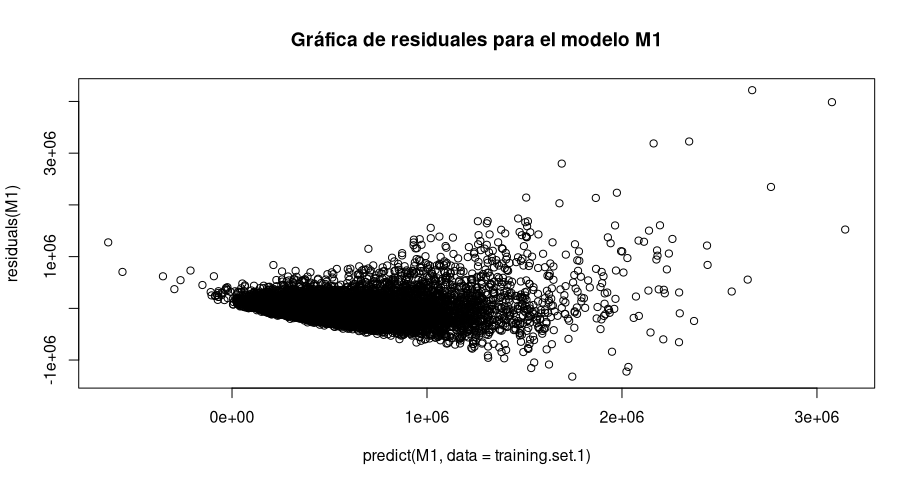
\includegraphics[scale=0.5]{residuals_m1.png}
	\caption{Residuales del modelo M1.}
	\label{fig:res_m1}
\end{figure}

Se plantean entonces algunas transformaciones para corregir este problema. En particular se consideraron las transformaciones cuadrática recíproca y Box Cox. Al modelo con la transformación $\sqrt{y}$ lo llamaremos $M2$, la modelo con la transformación $1/y$ lo llamaremos $M3$ y al modelo con la transformación $y^{\lambda}$ lo denominaremos $M4$. Las Figuras \ref{fig:res_m2}, \ref{fig:res_m3} y \ref{fig:res_m4} muestran los residuales para estos nuevos modelos. El valor de $\lambda$ máximo calculado con R es de $0.\bar{10}$

\begin{figure}[!htbp]
	\includegraphics[scale=0.5]{residuals_m2.png}
	\caption{Residuales del modelo M2.}
	\label{fig:res_m2}
\end{figure}

\begin{figure}[!htbp]
	\includegraphics[scale=0.5]{residuals_m3.png}
	\caption{Residuales del modelo M3.}
	\label{fig:res_m3}
\end{figure}

\begin{figure}[!htbp]
	\includegraphics[scale=0.5]{residuals_m4.png}
	\caption{Residuales del modelo M4.}
	\label{fig:res_m4}
\end{figure}

Estas gráficas muestran que los modelos $M2$ Y $M4$ muestran el comportamiento deseado. Sin embargo seleccionaremos el modelo $M4$ por tener mayor coeficiente de determinación.

\section{Diagnóstico}

\subsection{Normalidad de los residuales}
Para evaluar la normalidad de los residuales del modelo $M4$ utilizaremos una comprobación visual a través del q-q plot. A partir de la Figura \ref{fig:qqm4} podemos evidenciar un comportamiento normal en los residuales.

\begin{figure}[!htbp]
	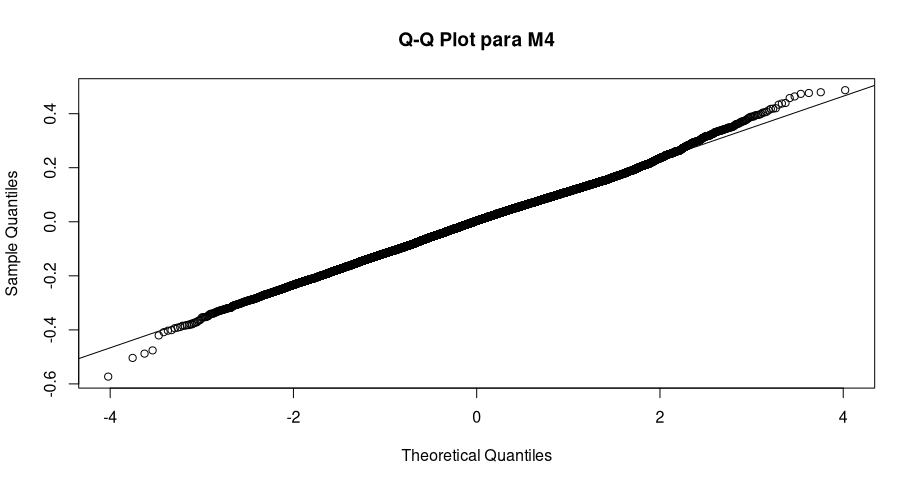
\includegraphics[scale=0.5]{qqplot_M4.png}
	\caption{Q-Q Plot para modelo M4.}
	\label{fig:qqm4}
\end{figure}

%\newpage
\subsection{Independencia de los errores}
Comprobaremos la independencia de los errores a través del test de Durbin-Watson. Este test arroja que $DW=2.033$ y $p=0.5851$. El valor de $p$ no permite rechazar la hipótesis nula que indica que no existe autocorrelación de primer orden. Es decir, puede que haga falta aplicar un modelo de regresión generalizado.

\subsection{Observaciones inusuales}

	\subsubsection{Valores atípicos}
El resultado del test de los p-valores de Bonferroni sugiere que la observación en la fila 13040 es la más extrema.

\begin{verbatim}
       rstudent unadjusted p-value Bonferroni p
13040 -4.937343         7.9933e-07      0.01382
\end{verbatim}

	\subsubsection{Observaciones con \textit{leverage}}
Para visualizar aquellos valores con alto \textit{leverage} utilizaremos el \textit{half normal plot} de la Figura \ref{fig:hfm4}. Aquí se evidencia que los registros 13627 y 3635 tienden a ejercer apalancamiento en los datos.

\begin{figure}[!htbp]
	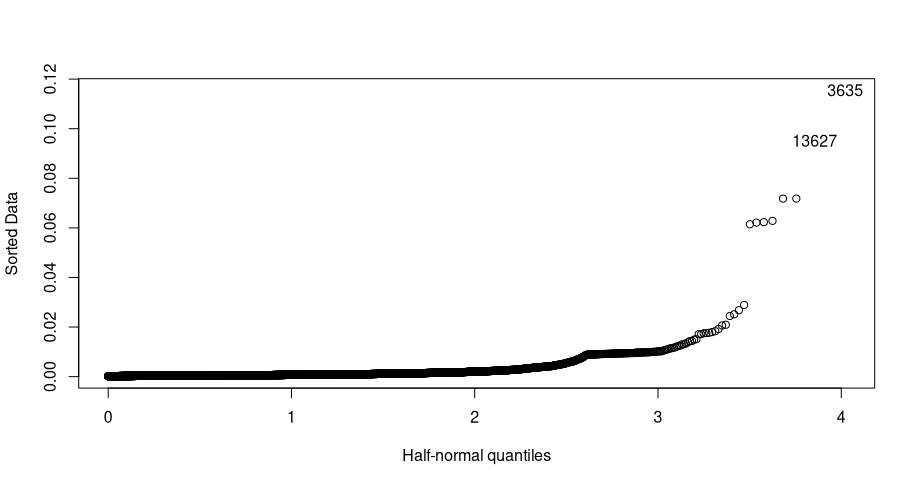
\includegraphics[scale=0.5]{hfm4.png}
	\caption{Q-Q Plot para modelo M4.}
	\label{fig:hfm4}
\end{figure}

	\subsubsection{Observaciones influyentes}
	Para identificar las observaciones más influyentes en el modelo se halla la distancia de Cook. La Figura \ref{fig:cookm4} no es muy clara en cuanto al efecto visual que debería generar.
	
	\begin{figure}[!htbp]
		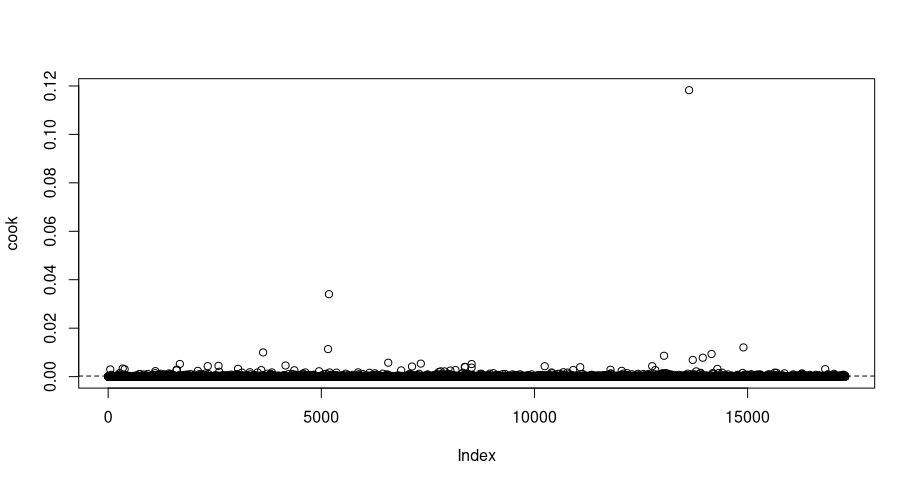
\includegraphics[scale=0.5]{cookm4.png}
		\caption{Distancia de Cook para modelo M4.}
		\label{fig:cookm4}
	\end{figure}
El gráfico de influencia de la Figura \ref{fig:infm4} arroja algo más de información con respecto a aquellas observaciones que más influyen en el modelo.
	\begin{figure}[!htbp]
		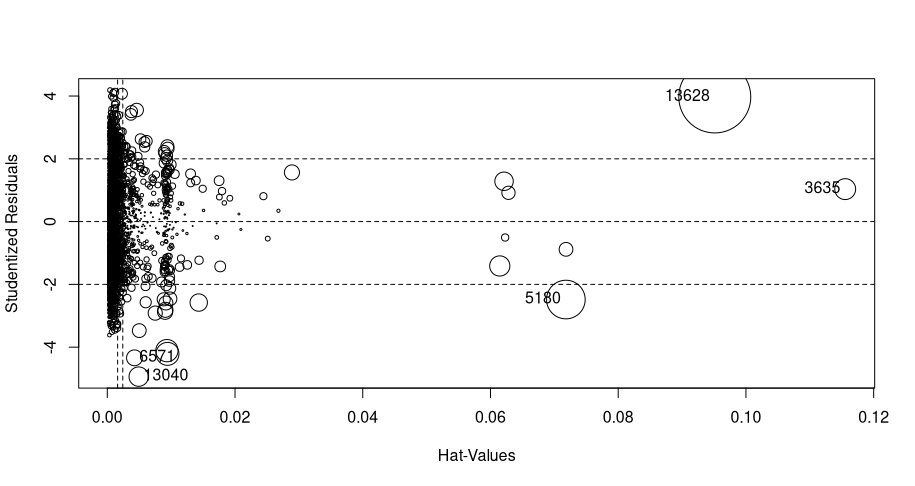
\includegraphics[scale=0.5]{infm4.png}
		\caption{Gráfico de influencia para modelo M4.}
		\label{fig:infm4}
	\end{figure}

\subsection{Verificación de la estructura del modelo}

EL Cuadro \ref{tab:cor} exhibe la matriz de correlación para el conjunto de datos depurado. Inicialmente no se evidencian altos niveles de correlación entre las variables. Aunque se hace llamativa la indagación entre la relación que pueda existir en las variables $x_3$ (\texttt{sqft\_living}) y $x_8$ (\texttt{sqft\_living15}), o $x_3$ (\texttt{sqft\_living}) y $x_{13}$ (\texttt{grade}).

% Matriz de correlación
\begin{table}[!htbp] \centering 
	\tiny 
	\begin{tabular}{@{\extracolsep{-7pt}} ccccccccccccccc} 
		\\[-1.8ex]\hline 
		\hline \\[-1.8ex] 
		& $y$ & $x_{1}$ & $x_{2}$ & $x_{3}$ & $x_{4}$ & $x_{5}$ & $x_{10}$ & $x_{11}$ & $x_{12}$ & $x_{13}$ & $x_{6}$ & $x_{7}$ & $x_{8}$ & $x_{9}$ \\ 
		\hline \\[-1.8ex] 
		$y$ & $1$ & $0.31$ & $0.52$ & $0.71$ & $0.09$ & $0.26$ & $0.26$ & $0.39$ & $0.03$ & $0.67$ & $$ & $0.06$ & $0.59$ & $0.08$ \\ 
		$x_{1}$ & $0.31$ & $1$ & $0.50$ & $0.57$ & $0.03$ & $0.17$ & $$-$0.01$ & $0.08$ & $0.03$ & $0.35$ & $$ & $0.14$ & $0.38$ & $0.02$ \\ 
		$x_{2}$ & $0.52$ & $0.50$ & $1$ & $0.75$ & $0.09$ & $0.50$ & $0.06$ & $0.19$ & $$-$0.13$ & $0.66$ & $$ & $0.50$ & $0.57$ & $0.09$ \\ 
		$x_{3}$ & $0.71$ & $0.57$ & $0.75$ & $1$ & $0.17$ & $0.36$ & $0.10$ & $0.28$ & $$-$0.06$ & $0.76$ & $$ & $0.32$ & $0.76$ & $0.18$ \\ 
		$x_{4}$ & $0.09$ & $0.03$ & $0.09$ & $0.17$ & $1$ & $0$ & $0.02$ & $0.06$ & $$-$0.01$ & $0.12$ & $$ & $0.06$ & $0.14$ & $0.73$ \\ 
		$x_{5}$ & $0.26$ & $0.17$ & $0.50$ & $0.36$ & $0$ & $1$ & $0.03$ & $0.04$ & $$-$0.27$ & $0.46$ & $$ & $0.49$ & $0.28$ & $$-$0.01$ \\ 
		$x_{10}$ & $0.26$ & $$-$0.01$ & $0.06$ & $0.10$ & $0.02$ & $0.03$ & $1$ & $0.38$ & $0.01$ & $0.08$ & $$ & $$-$0.02$ & $0.08$ & $0.03$ \\ 
		$x_{11}$ & $0.39$ & $0.08$ & $0.19$ & $0.28$ & $0.06$ & $0.04$ & $0.38$ & $1$ & $0.04$ & $0.25$ & $$ & $$-$0.05$ & $0.28$ & $0.06$ \\ 
		$x_{12}$ & $0.03$ & $0.03$ & $$-$0.13$ & $$-$0.06$ & $$-$0.01$ & $$-$0.27$ & $0.01$ & $0.04$ & $1$ & $$-$0.15$ & $$ & $$-$0.36$ & $$-$0.09$ & $$-$0.01$ \\ 
		$x_{13}$ & $0.67$ & $0.35$ & $0.66$ & $0.76$ & $0.12$ & $0.46$ & $0.08$ & $0.25$ & $$-$0.15$ & $1$ & $$ & $0.45$ & $0.72$ & $0.12$ \\ 
		$x_{6}$ & $$ & $$ & $$ & $$ & $$ & $$ & $$ & $$ & $$ & $$ & $1$ & $$ & $$ & $$ \\ 
		$x_{7}$ & $0.06$ & $0.14$ & $0.50$ & $0.32$ & $0.06$ & $0.49$ & $$-$0.02$ & $$-$0.05$ & $$-$0.36$ & $0.45$ & $$ & $1$ & $0.33$ & $0.07$ \\ 
		$x_{8}$ & $0.59$ & $0.38$ & $0.57$ & $0.76$ & $0.14$ & $0.28$ & $0.08$ & $0.28$ & $$-$0.09$ & $0.72$ & $$ & $0.33$ & $1$ & $0.18$ \\ 
		$x_{9}$ & $0.08$ & $0.02$ & $0.09$ & $0.18$ & $0.73$ & $$-$0.01$ & $0.03$ & $0.06$ & $$-$0.01$ & $0.12$ & $$ & $0.07$ & $0.18$ & $1$ \\ 
		\hline \\[-1.8ex] 
	\end{tabular} 
	\caption{Matriz de correlación} 
	\label{tab:cor} 
\end{table} 

El Cuadro \ref{tab:estr} muestra los gráficos de residuales parciales para cada variable. Esta gráfica sugiere que las variables \texttt{bedrooms}, \texttt{sqft\_lot}, \texttt{floors} y \texttt{condition} no deberían ser incluidas en el modelo, pues su efecto sobe la variable dependiente no se ajusta al de una línea recta.

\newpage
% PRPLOTS
\begin{table}%[!htbp]
	\centering
	\begin{tabular}{cc}
		\addheight{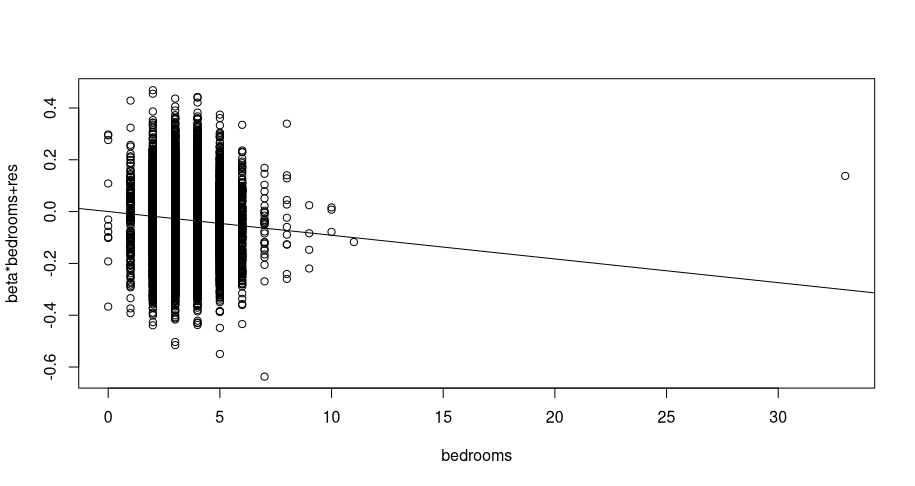
\includegraphics[width=45mm]{pr1.png}} &
		\addheight{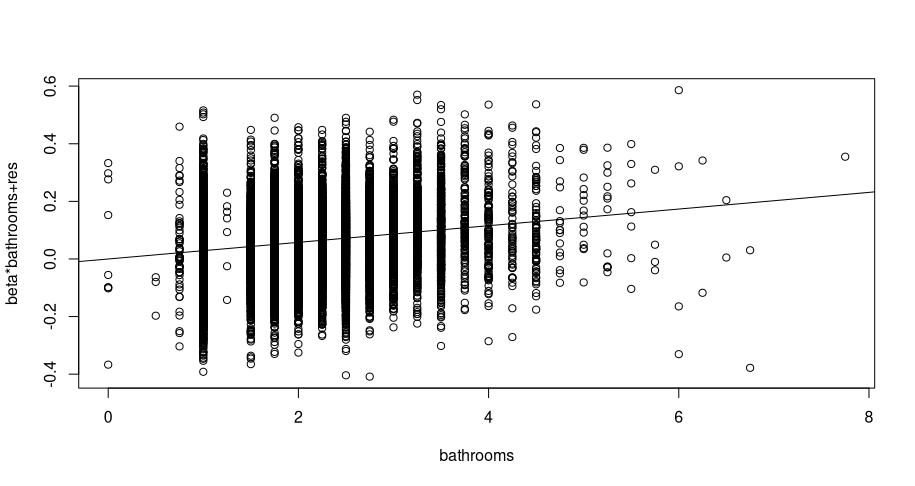
\includegraphics[width=45mm]{pr2.png}} \\
		\addheight{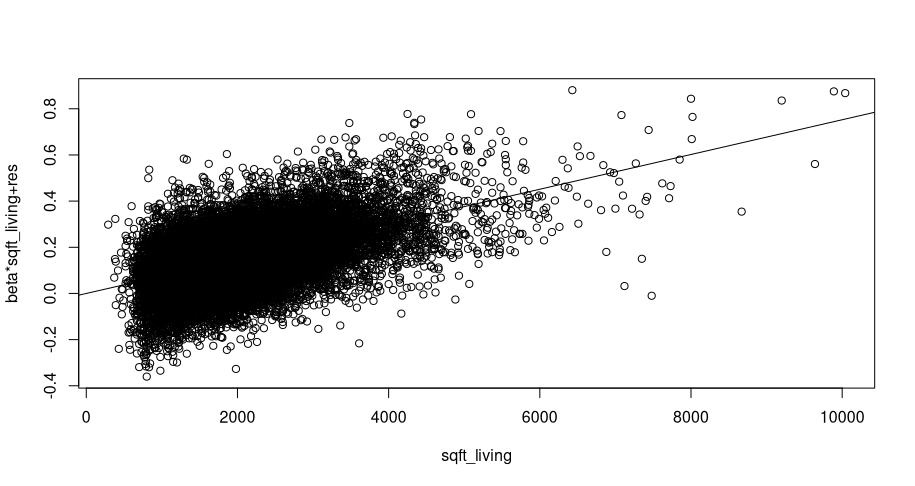
\includegraphics[width=45mm]{pr3.png}} &
		\addheight{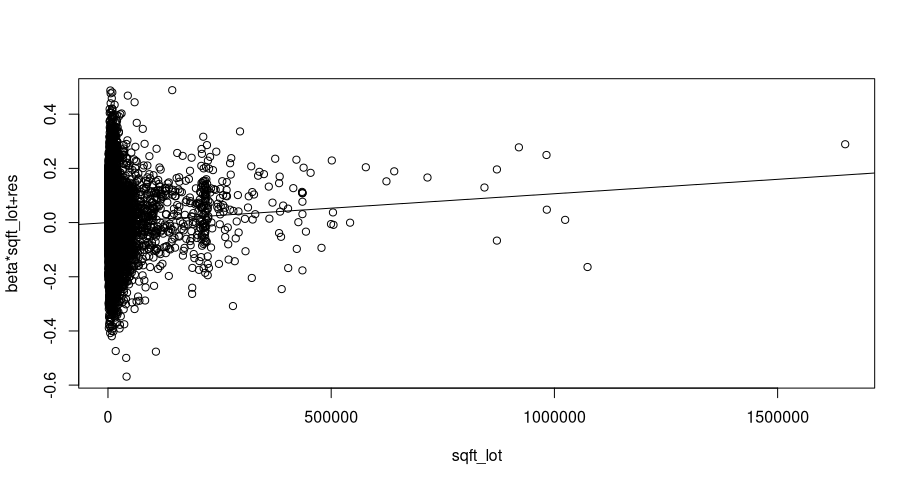
\includegraphics[width=45mm]{pr4.png}} \\
		\addheight{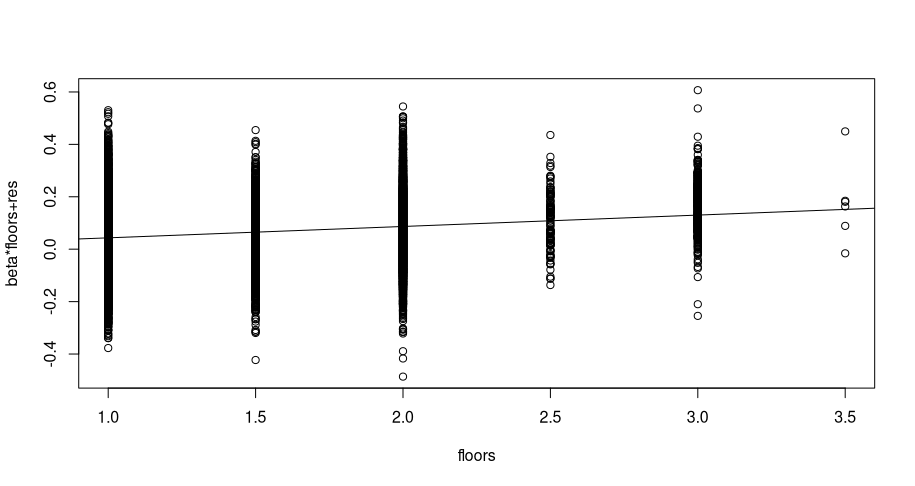
\includegraphics[width=45mm]{pr5.png}} &
		\addheight{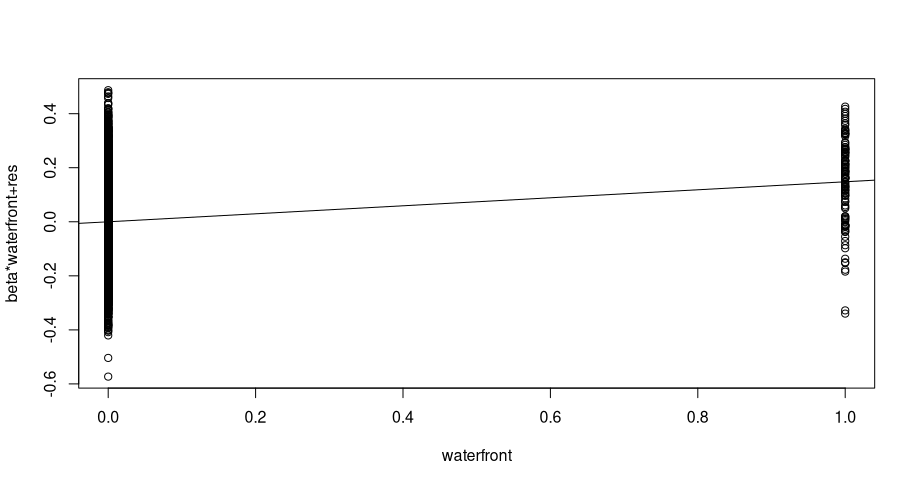
\includegraphics[width=45mm]{pr6.png}} \\
		\addheight{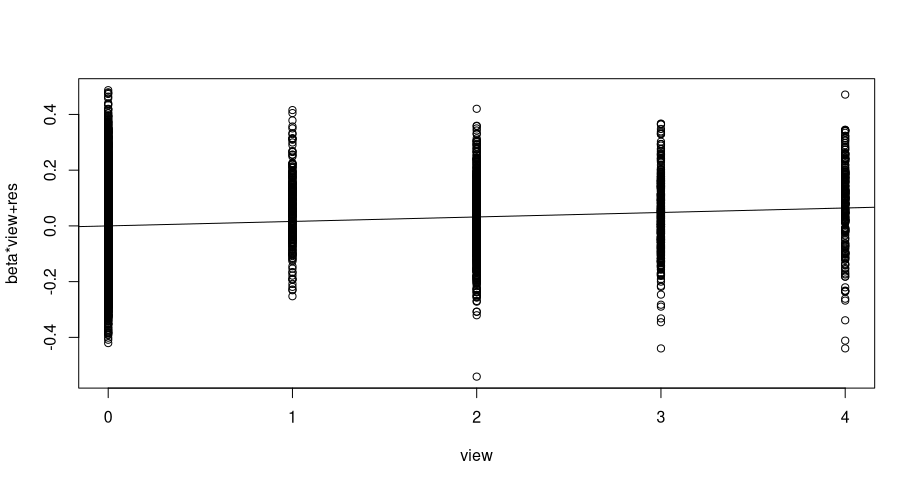
\includegraphics[width=45mm]{pr7.png}} &
		\addheight{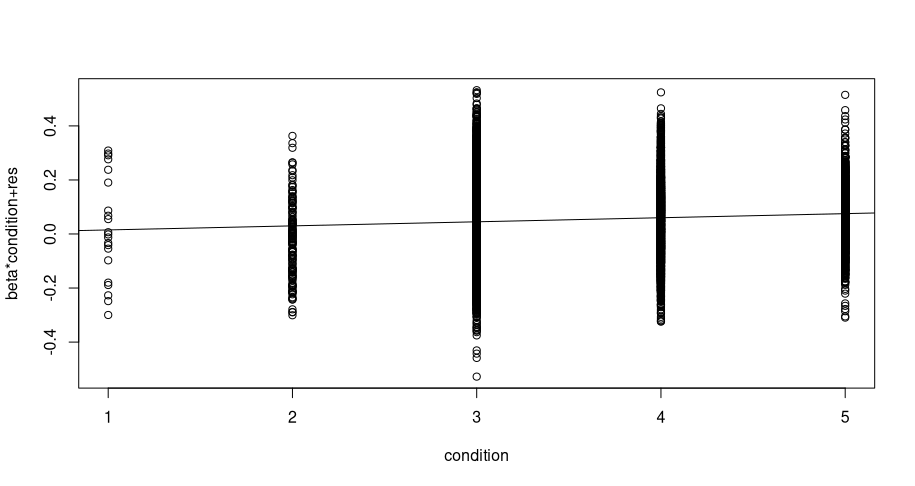
\includegraphics[width=45mm]{pr8.png}} \\
		\addheight{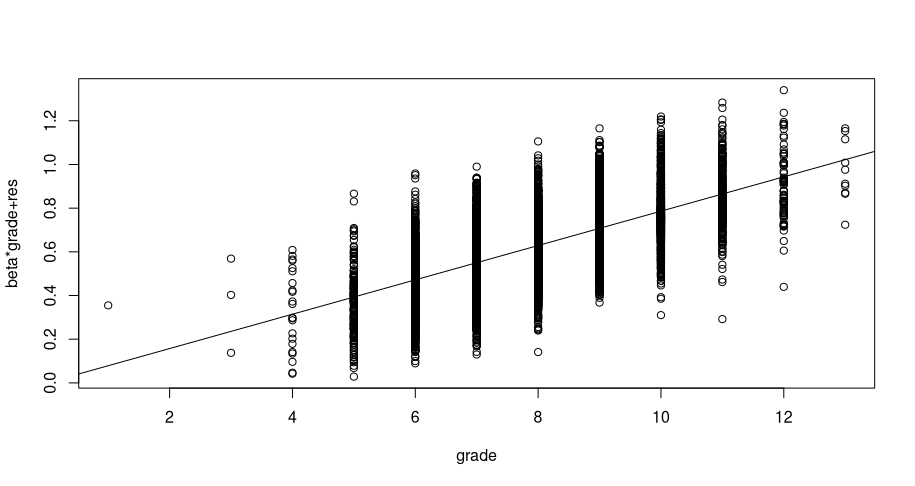
\includegraphics[width=45mm]{pr9.png}} &
		\addheight{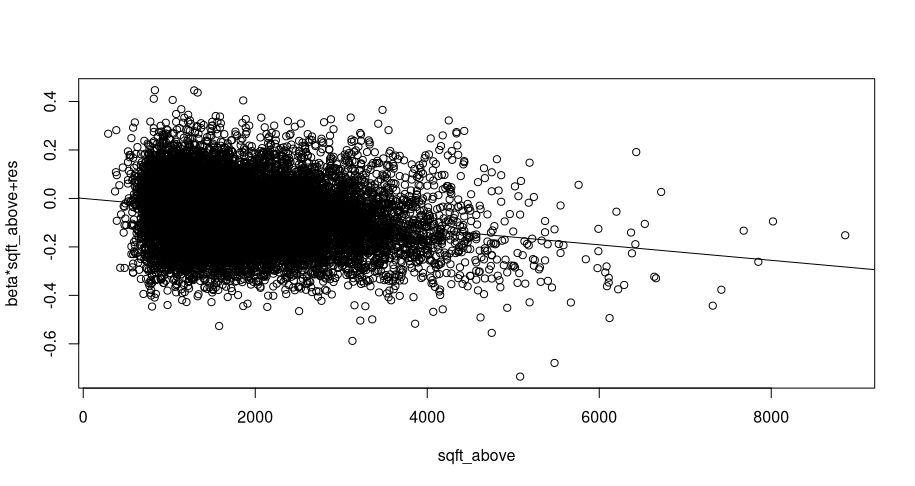
\includegraphics[width=45mm]{pr10.png}} \\
		\addheight{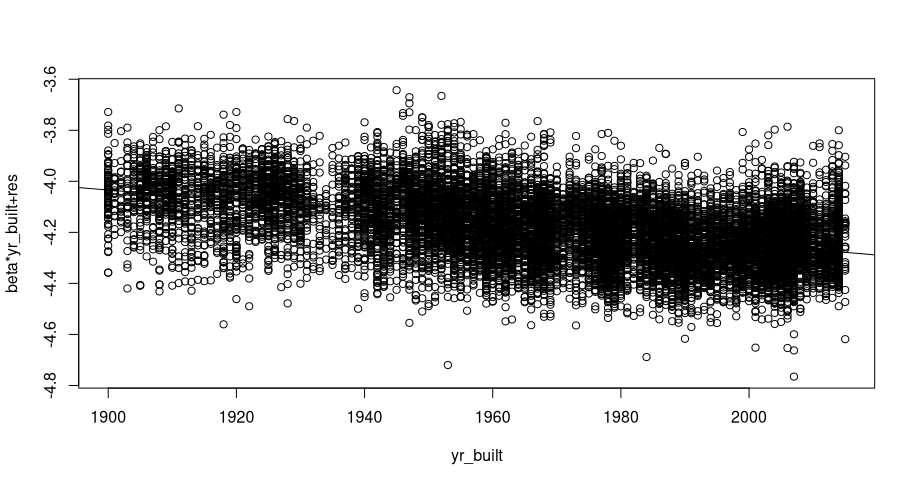
\includegraphics[width=45mm]{pr11.png}} &
		\addheight{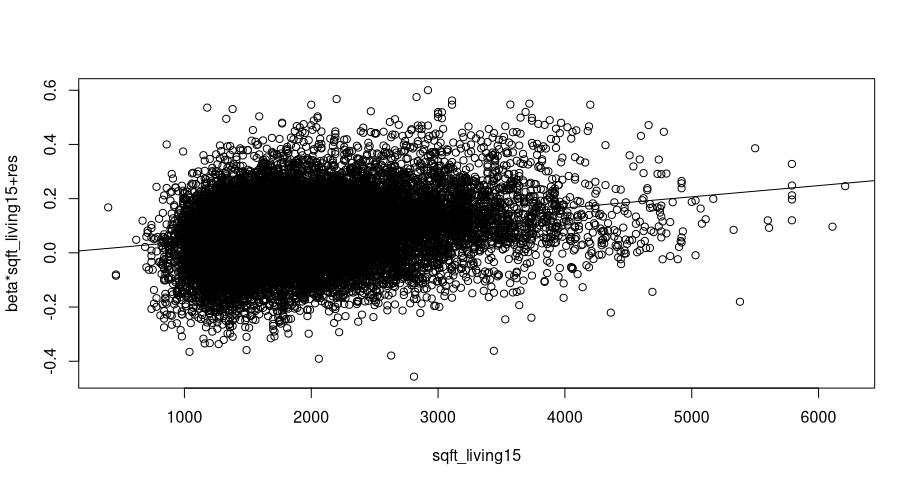
\includegraphics[width=45mm]{pr12.png}} \\
		\addheight{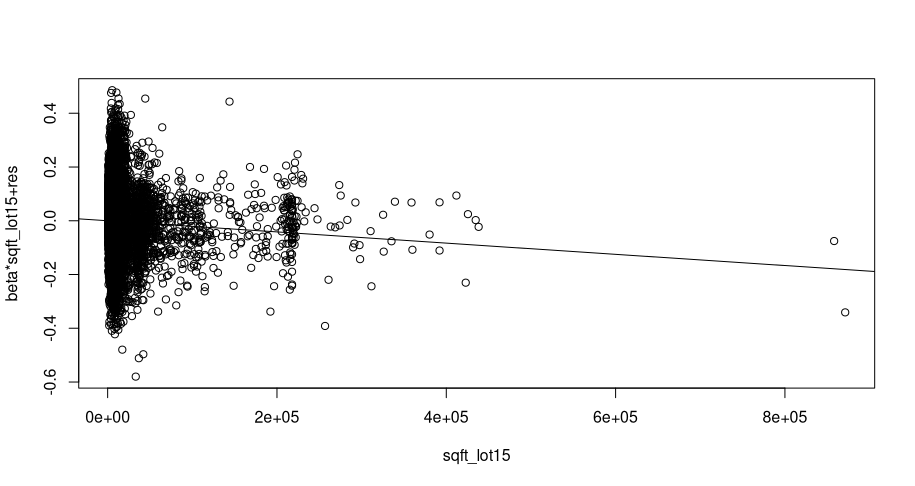
\includegraphics[width=45mm]{pr13.png}} & \\
	\end{tabular}
	\caption{Gráficas de residuales parciales para cada coeficiente.} 
	\label{tab:estr}
\end{table}

Para determinar si existe multicolinealidad entre las variables del modelo, calcularemos el factor de inflación de la varianca (VIF) para las variables. Al observar lel gráfico, se evidencia la fuerte correlación entre las variables \texttt{sqft\_above} y \texttt{sqft\_living}. En este caso, basándonos en la matriz de correlación del Cuadro \ref{tab:cor}, se puede descartar la variable \texttt{sqft\_living} al tener mayor correlación con el resto de variable y, por tanto, menor significancia estadística.

\begin{figure}[!htbp]
	\center
	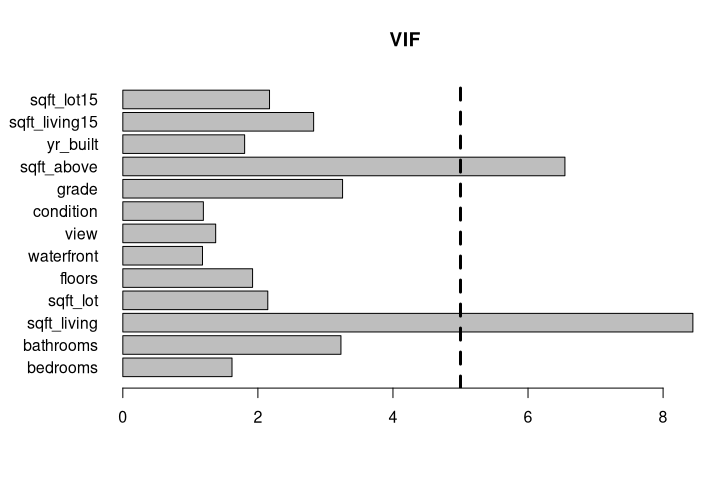
\includegraphics[scale=0.5]{vif.png}
	\caption{Factor de inflación de la varianza (VIF)}
	\label{fig:vif}
\end{figure}

Por último, evaluamos del cuadrado medio del error (RMSE) a través de la siguiente fórmula:

\[
RMSE = \sqrt{\frac
	{\sum_{i=1}^{n}{(\hat{Y}_i-Y_i)²}}
		{n}}
\]

Para el caso del modelo $M4$ este valor es 0.1163. Este valor indica que la diferencia entre los valores predichos y los reportados no es muy alta.


\end{document}